\documentclass[]{article}
\usepackage[margin=30mm]{geometry}
\usepackage{tikz}
\usepackage{todonotes}
\usepackage{fancyhdr}
\pagestyle{fancy}
\fancyhf{}
\rhead{Dilawar Singh}
\lhead{Habenula network}
\rfoot{Page \thepage}
\usetikzlibrary{calc,positioning,fit,arrows}
\title{Network of Habenula}
\author{Dilawar Singh}


\begin{document}

Synapse \tikz \draw[-*] (0,0) -- ++(.5,0); are excitatory, and synapse \tikz
\draw[-|,] (0,0) -- ++(.5,0); is inhibitory.

\section{Topology A}
\label{sec:1}

\begin{figure}[ht]
    \centering
    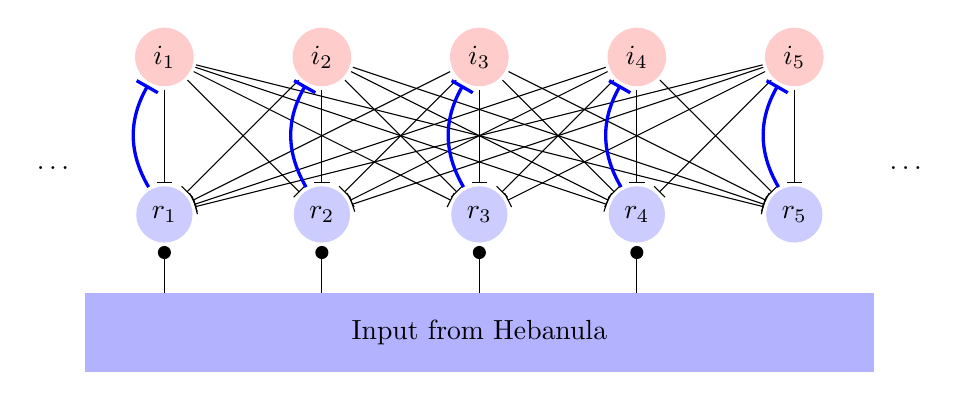
\begin{tikzpicture}[scale=1 
        , node distance = 2cm
        , every path/.style={ draw, outer sep=.5mm }
        , every node/.style={  } 
        ]

        \foreach \y in {1,2,3,4,5} 
            \node[draw=red!20,circle,fill=red!20] (i\y) at (2*\y,0) {$i_\y$};

        \foreach \y in {1,2,3,4,5}
            \node[draw=blue!20,circle,fill=blue!20] (r\y) at (2*\y,-2) {$r_\y$};

        \path[-|, ] (i1) edge (r1) edge (r2) edge (r3) edge (r4) edge (r5);
        
        \path[-|] (i2) edge[solid] (r1) edge[solid] (r2) edge[solid] (r3) 
            edge[solid] (r4) edge[solid] (r5);

        \path[-|, ] (i3) edge (r1) edge (r2) edge (r3) edge (r4) edge (r5);
        \path[-|, ] (i4) edge (r1) edge (r2) edge (r3) edge (r4) edge (r5);
        \path[-|, ] (i5) edge (r1) edge (r2) edge (r3) edge (r4) edge (r5);

        % Each raphe inhibits interneurons.
        \path[-|,blue, bend left,very thick] (r1) edge (i1)
                        (r2) edge (i2)
                        (r3) edge (i3)
                        (r4) edge (i4)
                        (r5) edge (i5)
                        ;

        % raphe interneurons gets excitatory input from other neuross.
        \draw[fill=blue!30,solid,draw=blue!30] (1,-4) rectangle (11, -3)
            node[pos=.5] (input) {Input from Hebanula}
            ;
        \draw[*-] (r1) -- ++(0,-1);
        \draw[*-] (r2) -- ++(0,-1);
        \draw[*-] (r3) -- ++(0,-1);
        \draw[*-] (r4) -- ++(0,-1);

        \node[below right of=i5] {$\ldots$};
        \node[below left of=i1] {$\ldots$};

    \end{tikzpicture}    
    \label{fig:1}
    \caption{A dense topology}
\end{figure}

\begin{figure}[h!]
\begin{center}
    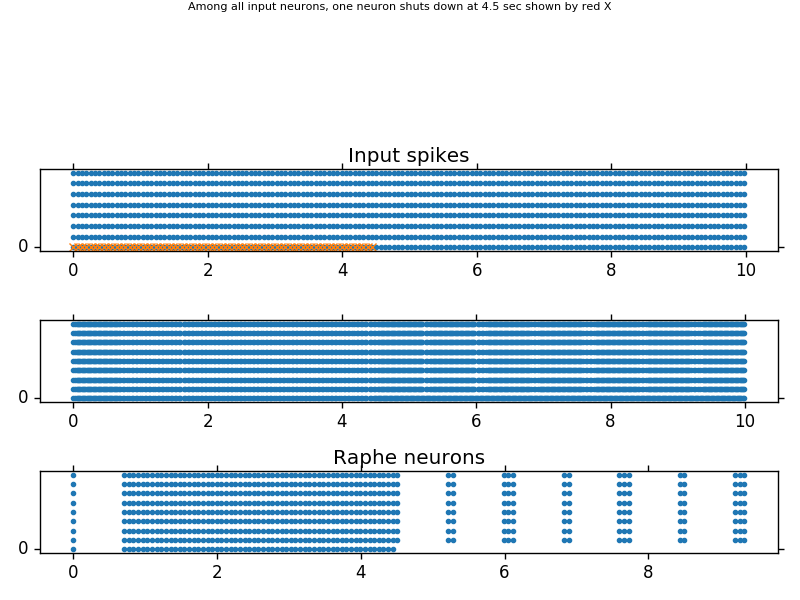
\includegraphics[width=1\textwidth]{./_snapshots/437f1834-d269-11e5-9456-e94c7dbd7a53.png}
\end{center}

\caption{Representative simulation of topology A. The initial part of simulation
    -- upto 1 seconds -- can be ignored. }
\label{fig:simulation}
\end{figure}

One representative simulation is shown in figure \ref{fig:simulation}.
\todo[inline]{I probably should do longer simulation}

The network shown in figure \ref{fig:1} shows right behaviour  but it is
probably not the best one. The interneurons in this model makes connections with
almost every other Raphe neuron. To overcome this, one can hypothesise that
interneurons makes excitatory connections to each other, and inhibitory
connections from interneurons to raphe are sparser. This topology is explored in
next section.

\section{Topology B}
\label{sec:2}

This topology is bit more realistic than topology A of section \ref{sec:1}.

In this network, the interneurons make excitatory connection onto other
interneurons in its neighbourhood of radius \footnote{radius $n$ means that
    $abs(i-j) <= n$ is satisfied where $i$ and $j$ are indices of interneurons.
} 2. Excitatory connections are necessary to spread the influence of a Raphe
neurons to other interneurons (since we don't connect to each Raphe neuron as we
did in topology A).

\begin{figure}[h!]
    \centering
    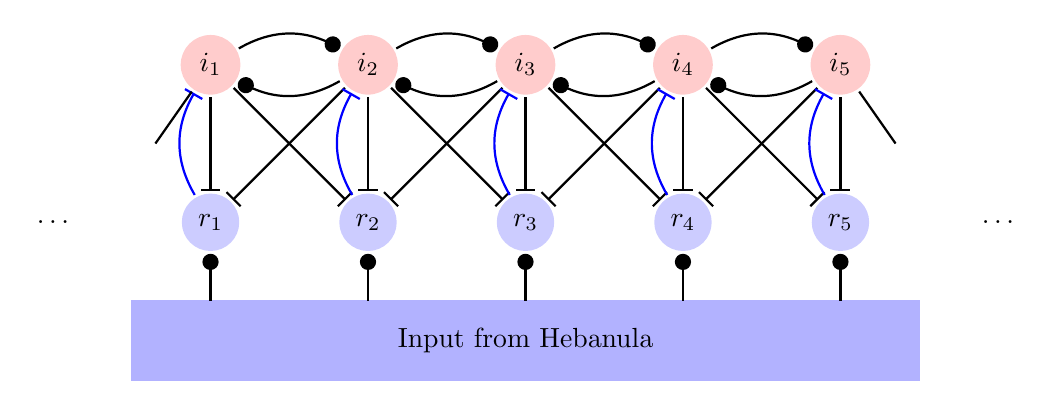
\begin{tikzpicture}[scale=1 
        , node distance = 2cm
        , every path/.style={ draw, thick, outer sep=.5mm }
        , every node/.style={  } 
        ]

        \foreach \y in {1,2,3,4,5} 
            \node[draw=red!20,circle,fill=red!20] (i\y) at (2*\y,0) {$i_\y$};

        \foreach \y in {1,2,3,4,5}
            \node[draw=blue!20,circle,fill=blue!20] (r\y) at (2*\y,-2) {$r_\y$};

        \node[right of=r5] (r6) {$\dots$};
        \node[left of=r1] (r0) {$\ldots$};

        \path[-|, ] (i1) edge (r1) edge (r2);
        
        \path[-|] (i2) edge (r1) edge (r2) edge (r3);

        \path[-|, ] (i3) edge (r2) edge (r3) edge (r4);
        \path[-|, ] (i4) edge (r3) edge (r4) edge (r5);
        \path[-|, ] (i5) edge (r4) edge (r5);

        % Each raphe inhibits interneurons.
        \path[-|,blue, bend left,very thick] (r1) edge (i1)
                        (r2) edge (i2)
                        (r3) edge (i3)
                        (r4) edge (i4)
                        (r5) edge (i5)
                        ;
        \draw[-] (i5) -- ++(0.7,-1);
        \draw[-] (i1) -- ++(-0.7,-1);

        % raphe interneurons gets excitatory input from other neuross.
        \draw[fill=blue!30,solid,draw=blue!30] (1,-4) rectangle (11, -3)
            node[pos=.5] (input) {Input from Hebanula}
            ;
        \draw[*-] (r1) -- ++(0,-1);
        \draw[*-] (r2) -- ++(0,-1);
        \draw[*-] (r3) -- ++(0,-1);
        \draw[*-] (r4) -- ++(0,-1);
        \draw[*-] (r5) -- ++(0,-1);

        % And interneurons make excitatory connections onto themselves.
        \draw[-*,bend left] (i1) edge (i2) 
                (i2) edge (i3)
                (i3) edge (i4) 
                (i4) edge (i5)
                ;

        \draw[-*,bend left] (i2) edge (i1)
                (i3) edge (i2)
                (i4) edge (i3)
                (i5) edge (i4)
                ;

    \end{tikzpicture}    
    \caption{}
    \label{fig:2}
\end{figure}

And a representative simulation of this topology is shown in figure
\ref{fig:simulation2}.

\begin{figure}[ht!]
\begin{center}
    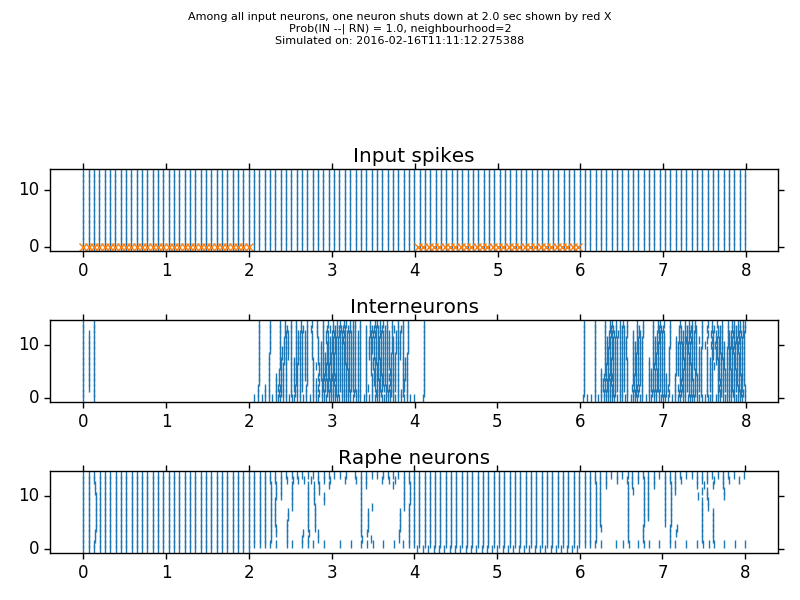
\includegraphics[width=1\textwidth]{./_snapshots/minimal_network.py.png}
\end{center}
\caption{}
\label{fig:}
\end{figure}



\end{document}
